\documentclass{article}

\usepackage{graphicx}
\usepackage{tikz}
\usepackage{tikzsymbols}
\usetikzlibrary{calc,patterns,shapes.geometric}
\pagestyle{empty}
\usepackage[margin=0pt]{geometry}
\geometry{papersize={14in,12in}}

\def\centerarc[#1](#2)(#3:#4:#5){\draw[#1] ($(#2)+({#5*cos(#3)},{#5*sin(#3)})$) arc (#3:#4:#5);}

\begin{document}
	\begin{figure}
		\centering
		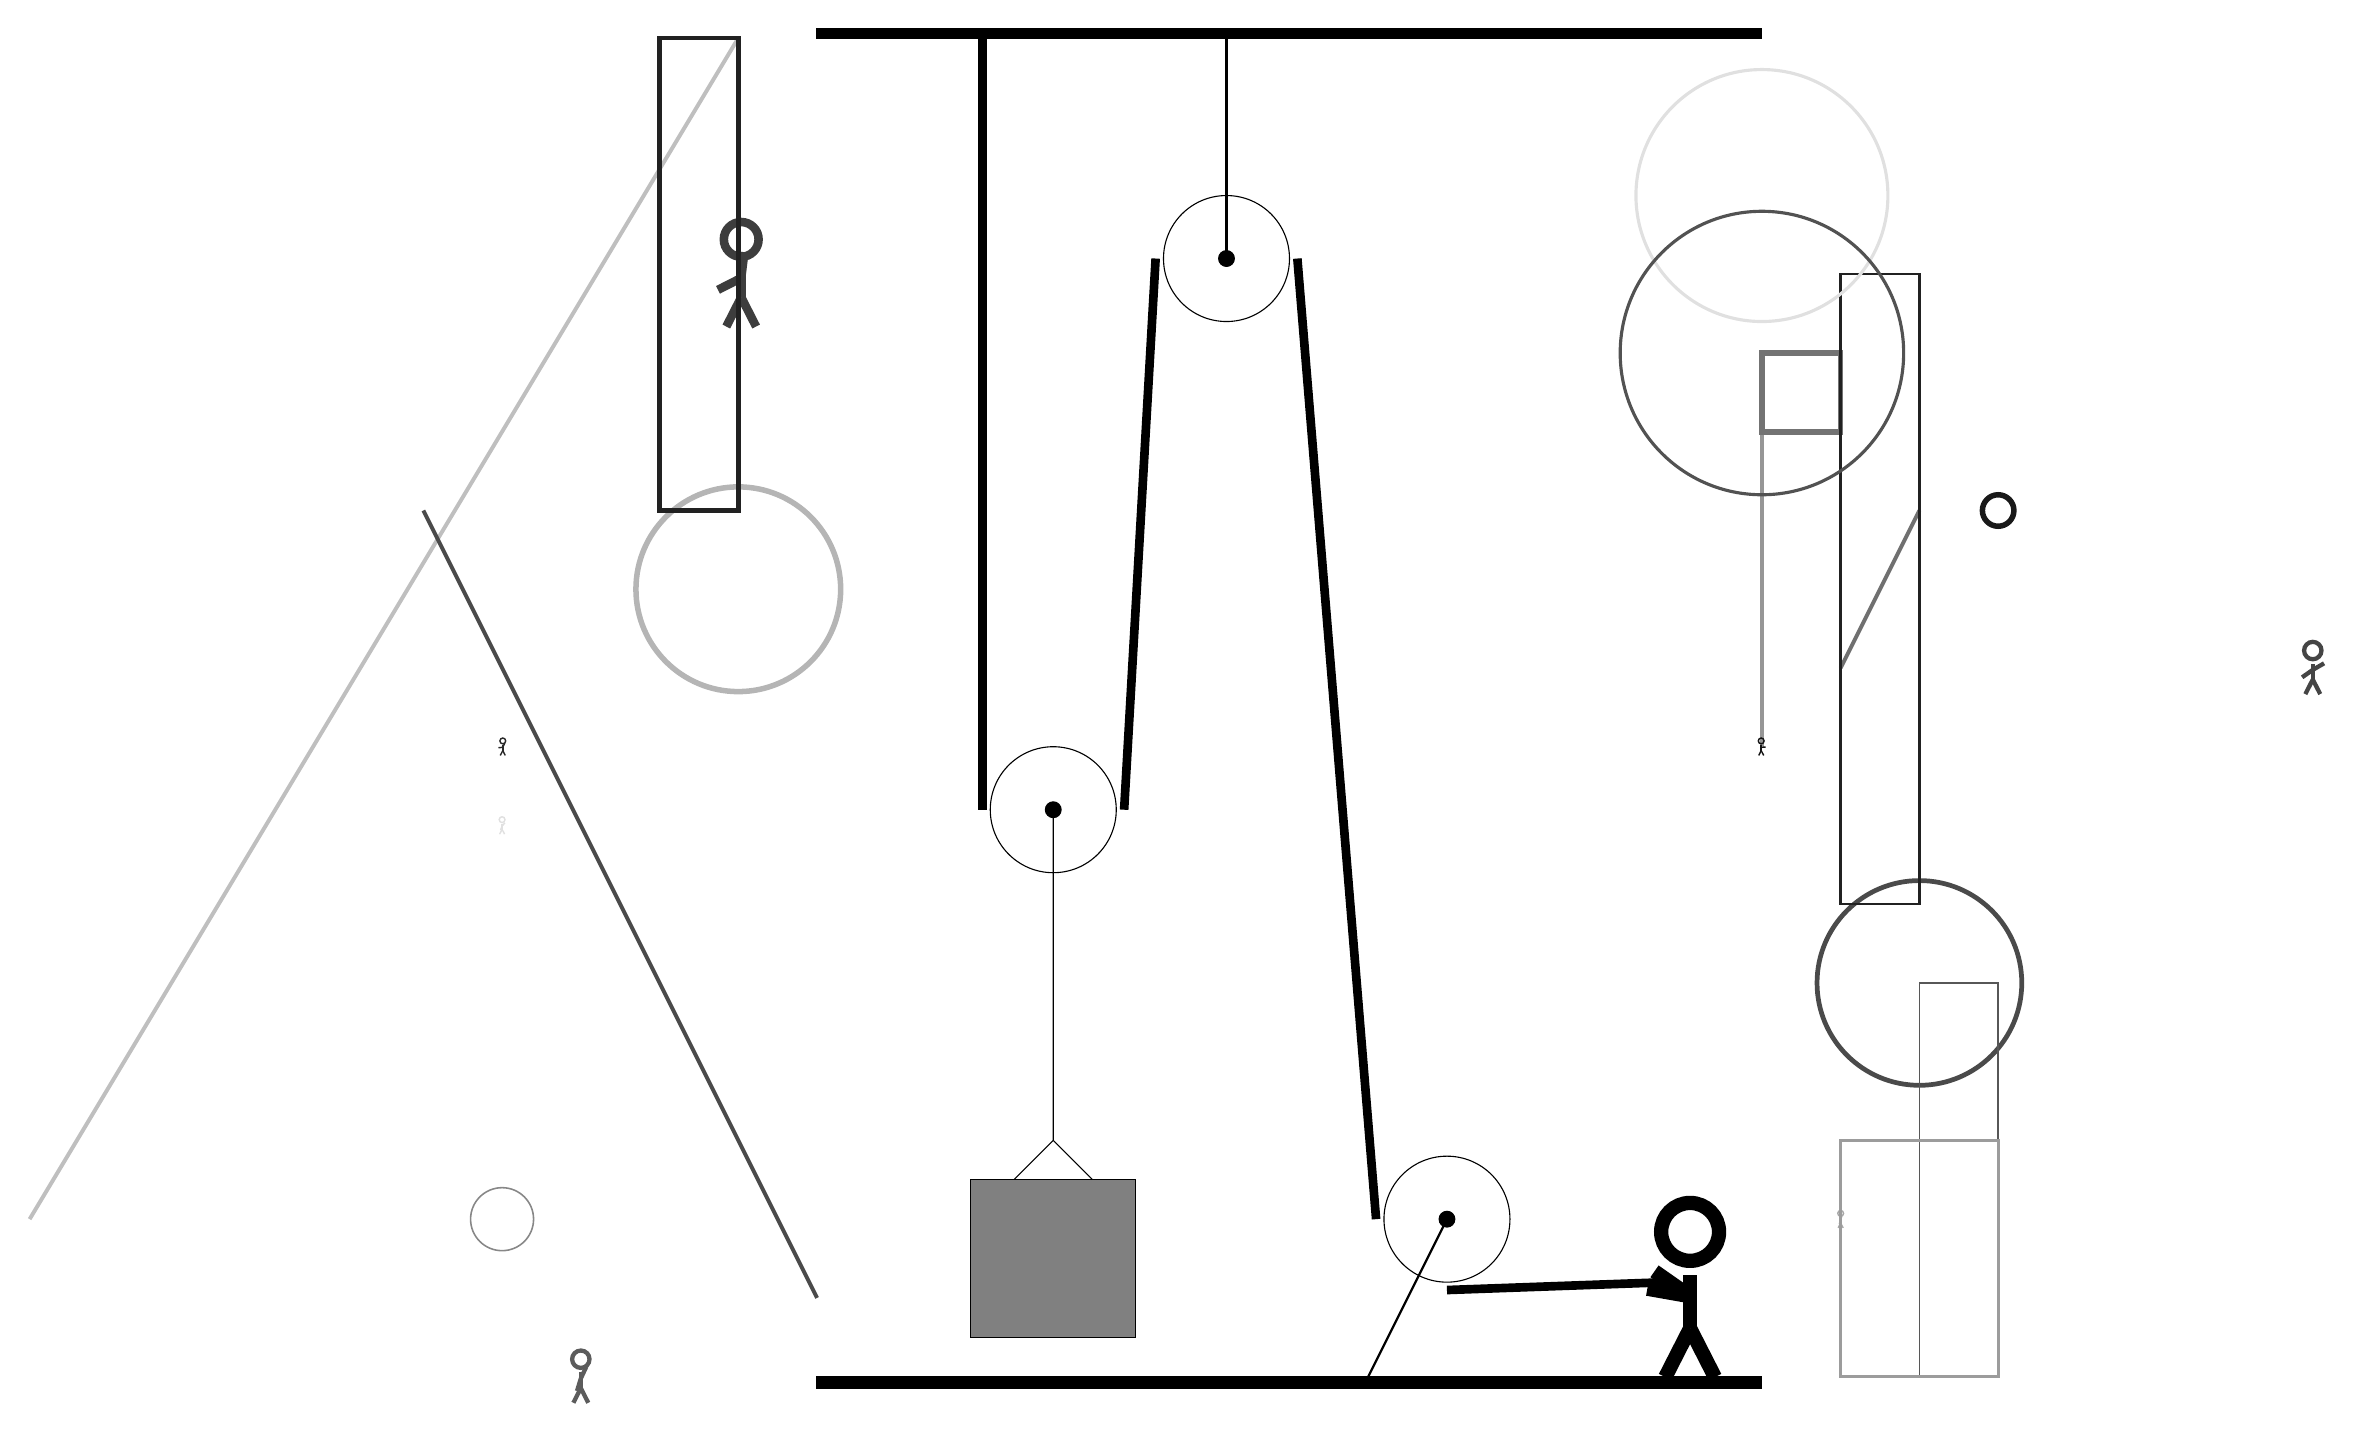
\begin{tikzpicture}
			%%%%% START %%%%%
			
			\draw[fill=black] (-2, 14) rectangle (10, 14.125);
			
			\draw (3.2, 11.2) circle (0.8);
			\draw[fill=black] (3.2, 11.2) circle (0.1);
			\draw[thick] (3.2, 11.2) -- (3.2, 14);
			
			\draw (6, -1) circle (0.8);
			\draw[fill=black] (6, -1) circle (0.1);
			\draw[thick] (6, -1) -- (5, -3);
			
			\draw (1, 4.2) circle (0.8);
			\draw[fill=black] (1, 4.2) circle (0.1);
			
			\draw[line width=0.5mm, color=black!56](11, 6) -- (12, 8);
			
			\draw [line width=0.6mm, color=black!71](12, 2) circle (1.3);
			\draw[line width=0.5mm, color=black!25](-3, 14) -- (-12, -1);
			\node[line width=0.5mm, color=black!34] at (11, -1) {\Strichmaxerl[1][72][73]};
			\node[line width=0.6mm, color=black!12] at (-6, 4) {\Strichmaxerl[1][69][49]};
			
			\draw[line width=0.5mm, color=black!41] (10, 10) rectangle (10, 5);
			\draw[line width=0.2mm, color=black!66] (12, -3) rectangle (13, 2);
			\draw[line width=0.7mm, color=black!55] (10, 9) rectangle (11, 10);
			\node[line width=0.3mm, color=black!84] at (-6, 5) {\Strichmaxerl[1][5][65]};
			\node[line width=0.5mm, color=black!76] at (-3, 11) {\Strichmaxerl[6][27][83]};
			\draw [line width=0.2mm, color=black!47](-6, -1) circle (0.4);
			\draw[line width=0.3mm, color=black!87] (11, 11) rectangle (12, 3);
			\draw [line width=0.4mm, color=black!12](10, 12) circle (1.6);
			
			\draw [line width=0.7mm, color=black!90](13, 8) circle (0.2);
			\draw [line width=0.4mm, color=black!68](10, 10) circle (1.8);
			\draw [line width=0.7mm, color=black!29](-3, 7) circle (1.3);
			\node[line width=0.6mm, color=black!73] at (17, 6) {\Strichmaxerl[3][35][30]};
			\draw[line width=0.5mm, color=black!71](-2, -2) -- (-7, 8);
			\node[line width=0.6mm, color=black!92] at (10, 5) {\Strichmaxerl[1][88][4]};
			
			\node[line width=0.3mm, color=black!64] at (-5, -3) {\Strichmaxerl[3][73][65]};
			\draw[line width=0.6mm, color=black!87] (-4, 8) rectangle (-3, 14);
			
			\draw[line width=0.4mm, color=black!39] (11, 0) rectangle (13, -3);
			
			
			\draw (1, 4.2) -- (1, 0) -- (0.5, -0.5);
			\draw (1, 0) -- (1.5, -0.5);
			\draw[fill=black!50] (-0.05, -0.5) rectangle (2.05, -2.5);
			
			\draw[line width=1.1mm] (0.1, 14) -- (0.1, 4.2);
			\centerarc[line width=1.1mm](1, 4.2)(180:360:0.9);
			\draw[line width=1.1mm](1.9, 4.2) -- (2.3, 11.2);
			\centerarc[line width=1.1mm](3.2, 11.2)(0:180:0.9);
			\draw[line width=1.1mm](4.1, 11.2) -- (5.1, -1);
			\centerarc[line width=1.1mm](6, -1)(180:270:0.9);
			\draw[line width=1.1mm](6, -1.9) -- (8.8, -1.8);
			
			\node at (9, -1.9) {\Strichmaxerl[10][-35][170]};
			
			\draw[fill=black] (-2, -3) rectangle (10, -3.15);
			
			%%%%% END %%%%%
		\end{tikzpicture}
	\end{figure}	
\end{document}